\documentclass[prodmode,acmtoms]{acmsmall}

\usepackage{listings}
\usepackage{graphicx}
\usepackage{psfrag}
\usepackage{amssymb}

%\usepackage{caption}
%\usepackage{subcaption}
%\usepackage{amsthm}

\usepackage{cite}
\usepackage[square]{natbib}
\usepackage{url}

%\newtheorem{theorem}{Theorem}

%\renewcommand\thesubfigure{Fig.\alph{subfigure}}



%opening

\markboth{M. Wang and M. Sitharam}{Algorithm xxx: Cayley analysis of mechanism configuration spaces using CayMos}
%\acmVolume{V}
%\acmNumber{N}
%\acmArticle{A}
%\acmYear{YYYY}
%\acmMonth{0}

\title{Algorithm xxx: Cayley Analysis of Mechanism Configuration Spaces using CayMos: 
Software Functionalities and Architecture }


%%% first author
\author{
MENGHAN WANG and MEERA SITHARAM 
\affil{University of Florida}
}

\begin{abstract}
For a common class of 2D mechanisms called \emph{1-dof tree decomposable linkages},
% we investigate the following fundamental problems:% have remained open:
%(a) How to canonically represent (and visualize) the connected components in the Euclidean realization space?
%(b) How to classify and efficiently find all the connected components,
%and the path(s) of continuous motion between two realizations in the same connected component, 
%with or without restricting the \emph{realization type} (sometimes called orientation type)?
%(c) How to efficiently find two realizations representing the shortest
%``distance" between two connected components?
we present a software package, \texttt{CayMos} %\cite{bib:caymos} 
which uses new theoretical results from Sitharam and Wang [2014] and Sitharam et al. [2011a,b]
%\cite{Sitharam2011a,Sitharam2011b,sitharam2014beast} 
to implement efficient algorithmic
solutions for: % the following problems:
(a) meaningfully representing and visualizing the connected components in the Euclidean realization space; 
%as (projections of) canonical Cayley curves; and
(b) %generating the connected components of the realization space, and 
finding a path of continuous motion  between two realizations in the same connected component,
with or without restricting the \emph{realization type} (sometimes called orientation type); 
% with time
%linear in a natural, discrete measure of the length of the path, as in
%\cite{Sitharam2011a,Sitharam2011b};
(c) finding two ``closest'' realizations in different connected components. 
%the realizations representing the shortest Cayley distance

\end{abstract}


\category{I.3.5}{Computational Geometry and Object Modeling}{Geometric algorithms, languages, and systems}
\terms{Algorithms}
\keywords{ 1-degree-of-freedom linkage, computer-aided design (CAD), motion space, realization space }
\acmformat{Menghan Wang and Meera Sitharam. 2014. Algorithm xxx: Cayley analysis of mechanism configuration spaces using CayMos: 
software functionalities and architecture.}

\begin{document}
\begin{bottomstuff}
This research was supported in part by the research grant NSF CCF-1117695
and a research gift from SolidWorks.
\end{bottomstuff}
\maketitle




\section{Introduction}


%BACKGROUND: cayley configuration space, 1-dof tree-decomposable linkages, continuous paths, 
%connected components


A key underlying barrier in understanding underconstrained geometric
constraint systems is the classical problem of representing and efficiently finding 
 the \emph{Euclidean realization spaces} of
\emph{1-degree-of-freedom linkages}, or \emph{mechanisms} in 2D.
A {\em linkage} $(G,\bar{l})$, is a graph $G=(V,E)$ with fixed
length bars as edges, i.e. $\bar{l}: E \rightarrow \mathbb{R}$. 
A 2D \emph{Euclidean realization} or \emph{configuration} $G(p)$ of $(G,\bar{l})$ is 
an assignment of points $p: V \rightarrow \mathbb{R}^2$ to the vertices of $G$ satisfying the bar lengths in $\bar{l}$, 
modulo Euclidean motions. 
If the linkage is \emph{flexible} (i.e., the space of realizations of a
linkage is infinite), but the addition of a
single bar causes the linkage to become \emph{minimally rigid} 
(i.e. only finitely many realizations), then the linkage is called a 
\emph{mechanism} with \emph{1-degree-of-freedom (1-dof)}. 
%A well-known example is the 2D mechanism underlying the Strandbeest, 
%shown in Figure \ref{fig:beest}. 




Describing and analyzing realization spaces of 1-dof linkages in 2D is 
a  difficult problem with a long history. 
%In mechanical computer aided design, it represents a key underlying barrier
%to understanding underconstrained geometric constraint system.
In fact, even for rigid linkages, the number of realizations can be exponential in the number of vertices
and not easy to estimate \citep{Borcea2004}. 
%One way to classify realizations is to use \emph{realization types} \cite{bib:navigation,bib:FudHo97},  
%which uniquely determines a realization of a rigid linkage. 
For flexible linkages, 
a well-known early result \citep{Kempe1875} 
shows that an arbitrary algebraic curve can be traced by the motion of a linkage joint. 
One outstanding example is the Peaucellier-Lipkin linkage, which transforms planar rotary motion into straight-line motion \citep{Kempe1877}. 
%For polygonal linkages, recent results on the variants of Carpenter's rule problem and pseudotriangulations yield spaces of non-crossing realizations and expansive motions \cite{bib:streinu05,bib:straightening,bib:rote03}.
Versions of the problem play an important role in Computer-Aided-Design (CAD), 
robotics and molecular geometry \citep{Sacks2010,Ying1995,Sitharam2005}, but few results are known beyond individual or specific families of linkages. 

\noindent{\bf Note:} In the remainder of this article the term ``linkage" refers specifically to ``2D linkage". 


In this paper, we restrict ourselves to \emph{1-dof tree-decomposable linkages}.
The underlying graphs $G$ of such linkages 
are obtained by dropping an edge from so-called \emph{tree-decomposable graphs}. 
Tree-decomposable linkages are 
minimally rigid and well-studied, for example, in geometric constraint solving and CAD.
For tree-decomposable linkages, if the bar lengths $\bar{l}$ are in $\mathbb{Q}$, 
the coordinate values of a realization are solutions to 
a triangularized quadratic system with coefficients in $\mathbb{Q}$
(i.e. the coordinates of the realization belong to an extension field over $\mathbb{Q}$ obtained by nested square-roots). 
Such values are called ruler-and-compass solvable or \emph{quadratically-radically solvable} \emph{(QRS)} values.
%because they are ruler-and-compass realizable or \emph{quadratically-radically solvable} (\emph{QRS}),
%i.e., if the bar lengths $\bar{l}$ are in $\mathbb{Q}$, the realizations are solutions to a
%triangularized quadratic system with coefficients in $\mathbb{Q}$
%(i.e. the coordinates of the realization belong to an extension field over
%$\mathbb{Q}$ obtained by nested square-roots). % and 

\begin{figure}

\psfrag{f}{$f$} 
\psfrag{0}{$v_0$}\psfrag{0'}{$v_{0}'$}
\psfrag{1}{$v_1$}\psfrag{2}{$v_2$}\psfrag{3}{$v_3$}\psfrag{4}{$v_4$}
\psfrag{a}{$u_1$} \psfrag{b}{$u_2$}
\psfrag{f2}{$f_2$}\psfrag{f3}{$f_3$}\psfrag{f4}{$f_4$}
\centering

\begin{minipage}{.33\linewidth}%
  \centering
  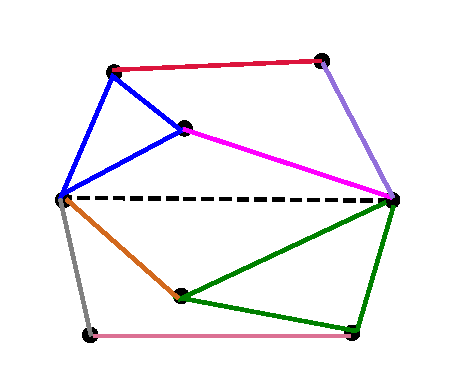
\includegraphics[width=.9\linewidth]{img/low}
  \label{fig:sub1}
  (a)
\end{minipage}%
\begin{minipage}{.33\linewidth}%
  \centering
  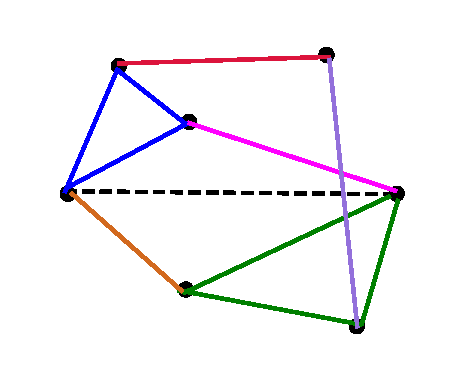
\includegraphics[width=.9\linewidth]{img/notlow}
  \label{fig:sub2}
  (b)
\end{minipage}%
\begin{minipage}{.33\linewidth}%
  \centering
  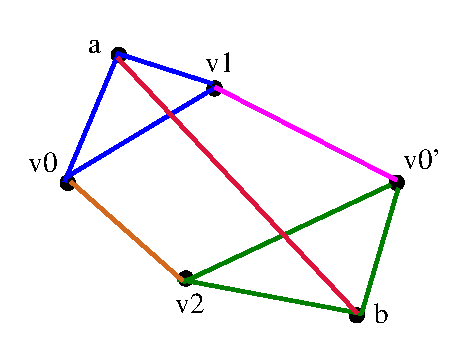
\includegraphics[width=.9\linewidth]{img/nott}
  \label{fig:sub3}
   (c)
\end{minipage}%


%\begin{subfigure}{.33\linewidth}
%  \centering
%  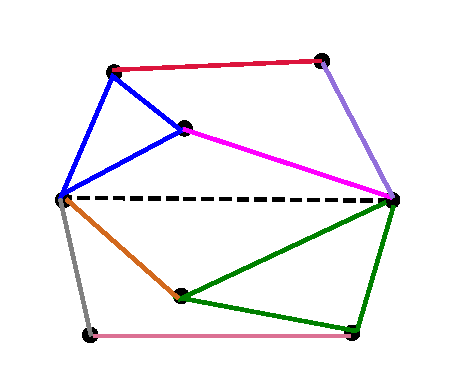
\includegraphics[width=.9\linewidth]{img/low}
%  \caption{}
%  \label{fig:sub1}
%\end{subfigure}%
%\begin{subfigure}{.33\linewidth}
%  \centering
%  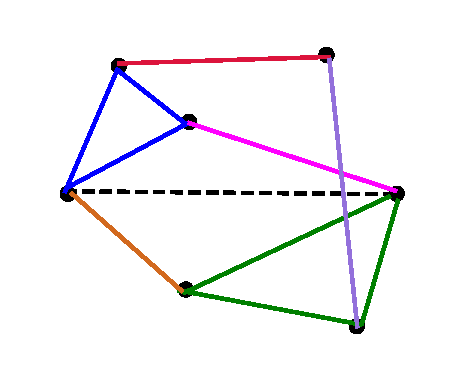
\includegraphics[width=.9\linewidth]{img/notlow}
%  \caption{}
%  \label{fig:sub2}
%\end{subfigure}
%\begin{subfigure}{.33\linewidth}
%  \centering
%  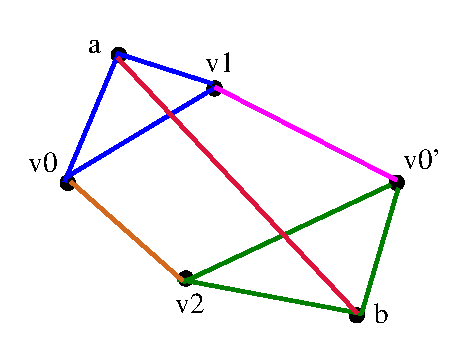
\includegraphics[width=.9\linewidth]{img/nott}
%  \caption{}
%  \label{fig:sub3}
%\end{subfigure}

\caption{ 
(a) A 1-dof tree-decomposable  linkage with low Cayley complexity (satisfies the Four-cycle Theorem). 
%: clusters $T_1T_2T_3T_4$ form a base four-cycle for construction step $v_k \triangleleft (u_k,w_k)$. 
(b)  A 1-dof tree-decomposable  linkage without low Cayley complexity (does not satisfy the Four-cycle Theorem).  
%For Definition \ref{def:complete_cayley}: the complete Cayley base non-edges for a linkage
%with three construction steps.
(c) A linkage that is not 1-dof tree-decomposable.
}

\label{fig:four_cycle}

\end{figure}

A graph $G$ is \emph{1-dof tree-decomposable} if there exists a non-edge $f$, 
called a \emph{base non-edge} (there could be more than one), 
such that $G$ has the following graph theoretical construction from $f$:
%(see for example Figure \ref{fig:beest}(a)):
at {\emph{Construction Step $k$}}, 
the graph constructed so far, $G_{k-1}$, is extended by
adding two new maximal tree-decomposable subgraphs, or \emph{clusters} $C_{k1}$ and $C_{k2}$ sharing a vertex $v_{k}$. 
In addition, $C_{k1}$ and $C_{k2}$ each has exactly one shared vertex, $u_k$ and $w_k$ respectively, 
with $G_{k-1}$. Such a construction step is denoted $v_k \triangleleft (u_k,w_k)$.
For example, the underlying graph of the linkage in Figure \ref{fig:four_cycle}(b) has three construction steps from the non-edge $f$:
$v_1 \triangleleft (v_0,v_0')$ which appends $\triangle v_0v_1a$ and the edge $(v_0',v_1)$,
$v_2 \triangleleft (v_0,v_0')$ which appends the edge $(v_0,v_2)$ and  $\triangle v_0'v_2b$, 
and $v_3 \triangleleft (a,b)$ which appends two edges $(v_3, a)$ and $(v_3, b)$.
Similarly, the underlying graph of the linkage in Figure \ref{fig:four_cycle}(a) has four construction steps from the non-edge $f$.
On the other hand, the underlying graph of the linkage in Figure \ref{fig:four_cycle}(c) is not 1-dof tree-decomposable, as there does not exist a construction sequence from any non-edge. 

A \emph{realization type} for a 1-dof tree-decomposable linkage 
specifies a \emph{local orientation} for the triple $(v_k,u_k,w_k)$,
for each construction step  $v_k \triangleleft (u_k,w_k)$. 
For example, for the linkage in Figure \ref{fig:four_cycle}(b), 
the construction step $v_3 \triangleleft (a,b)$ has a local orientation such that $a,b,v_3$ lie in counterclockwise order. Another possible orientation, with $a,b,v_3$ in clockwise order, can be obtained by flipping $v_3$ to the other side of $(a,b)$. 
For a given realization type, 
a 1-dof tree-decomposable linkage $(G,\bar{l})$ has a simple ruler and compass realization $G(p)$
which parallels the graph theoretic construction. 
%For example, for the linkage in Figure \ref{fig:beest}(a), the ruler and compass realization step corresponding to Construction Step 1 has two possible local orientations, 
%one is shown in the figure, and the other has $p(v_6)$ located on the other side of $(p(v_0),p(v_3))$. 
%The local orientations for all realization steps constitute the forward realization type. 
On the other hand, when a realization type is not specified, 
determining the existence of a realization is however NP-hard \citep{Sacks2010}. 


We note here that each cluster has finitely many realizations according to its inner realization types. 
As no continuous motion is possible between those realizations, 
in this paper, we assume that the clusters are \emph{globally rigid}, i.e. we fix the inner realization type of each cluster so that each cluster has a single realization. 
We also reduce clusters sharing only two vertices with the rest of the graph into edges. 









\subsection{Problems with the state of the art} \label{sec:soa}

There are numerous existing %examples of algorithms and 
softwares suites dealing with 1-dof tree-decomposable linkages, 
such as Geometry Expressions \citep{todd2007geometry}, SAM \citep{artasengineering2010sam},  Phun \citep{algoryx2013algodoo}, Sketchpad \citep{keycurriculum1995geometer}, Geogebra \citep{geogebrainc2001geogebra}, D-cubed \citep{siemens1999d},  GIM \citep{petuya2014educational}, CUIK \citep{porta2014open}, 
% the algorithm in \cite{Hidalgo2011}, 
etc. 
They have the following major functionalities: 
(\romannumeral 1) designing 1-dof tree-decomposable linkages for tracing out specific curves, 
especially by building new mechanisms based on a library of existing ones;
%Some of them provide a library of well-known mechanisms, so that the user
%can build new mechanisms based on the existing ones. 
%Focus on design linkages, especially based on well-known templates. 
(\romannumeral 2) accepting user-specified parameters, ranges and realization types to generate 
continuous motion of the linkages. 
%and allow user to trace various parameters of the linkage during continuous motion, 
%for example, the length of a base non-edge, the 2D curve traced out by a vertex, etc.

\smallskip
%However, the following issues, while already having some theoretical answers (which we will refer to in the next subsection), still have not been implemented. \\
However, while some theoretical answers have been provided recently for the following issues (which will be described in the next subsection), until now there has been no theoretically guaranteed software implementation that addresses these issues.

\noindent\textbf{(a)} How do we canonically represent and visualize the connected components? 
In the above softwares, 
the realization space is typically represented as separate curves in 2D that are 
traced by each vertex of the linkage. 
In fact, 
a realization actually corresponds to a tuple of points, one on each of these curves.
I.e., the realization space is bijectively represented by a curve in the full %, minimal 
\emph{ambient dimension} of $2|V|-3$ after factoring out rigid transformations, 
where $|V|$ is the number of vertices in the linkage. \\
\textbf{(b)} %Generating all connected components: 
%currently, there is no 
How do we generate all connected components  efficiently  and  how do we find a path of continuous motion between two arbitrary input realizations
in the same connected component? 
In order to generate continuous motion in most of the existing software suites except for CUIK,
%Until now, in order to generate continuous motion, 
the user must %fix the portion of the realization space of interest, 
specify a range of a parameter containing the parameter value at the given realization.
% to generate continuous motion. 
Then either a single connected component is generated
for a subset of the specified range, 
or multiple segments of the realization space, under only the given realization type,  
are generated within the specified range. We discuss this issue in more detail in the following subsection. \\
\textbf{(c)} How do we find the ``distance'' between connected components? 
Until now, 
for two realizations in different connected components, 
there is no software that finds how ``close" they can get towards each other by continuous motion, 
%between two realizations in different connected components of the realization space.
using a meaningful definition of ``distance" between connected components. 
%We discuss this issue in more detail at the end of Section \ref{sec:previous_cayley}.
%so continuous motion is generated
%within a fixed connected component of the realization space, 
%or within a fixed realization type.
%In \cite{Hidalgo2011}, an algorithm was developed to find a continuous
%motion path between two realizations for 1-dof tree-decomposable linkages.
%However, this algorithm requires exhaustive searching, and can have exponential time complexity
%even as a function of natural discrete measures of path lengths. \\
%We would like to generate the entire set of complete connected components of a linkage. \\
  %When analyzing the motion space, 
%According to different softwares, 



In this paper, we provide a theoretically guaranteed  software implementation to solve the above problems for 
 a natural and commonly occurring subclass of 1-dof tree-decomposable linkages. % called linkages with \emph{low Cayley complexity}.
%Our previous theoretical results \citep{Sitharam2011a} implies that
We also show that for any class of linkages larger than  this particular subclass, %linkages with low Cayley complexity, 
heuristic approaches adopted by existing software suites are necessarily intractable or incomplete. 
%and provide a theoretically provable software implementationthis subclass. 
%that have \emph{low Cayley complexity}. 
%The following subsection provides the required background. % concepts. % related to low Cayley complexity. 
%%


\subsection{Previous work on Cayley configuration spaces of 1-dof 2D linkages}
\label{sec:previous_cayley}


The recent papers \citeN{Sitharam2011a,Sitharam2011b,sitharam2014beast}
introduced the use of \emph{Cayley configuration space} to describe the 
realization space of a 1-dof, 2D linkage $(G,\bar{l})$.  
A Cayley configuration space is obtained by taking %a pair of vertices whose distance is not fixed by the bars,
%i.e., 
an {\em independent non-edge} $f$ with $G\cup f$ being minimally rigid, 
and asking for all possible lengths that $f$ can attain %\cite{Gao2005,Sitharam2008,Sitharam2011a,Sitharam2011b}
(\romannumeral 1) over all the realizations of $(G, \bar{l})$; 
(\romannumeral 2) over all realizations of $(G, \bar{l})$ of a particular realization type. % from $f$. 
For (\romannumeral 1) (resp. (\romannumeral 2)), each realizable length of $f$ is called a (resp. \emph{oriented}) \emph{Cayley configuration}, 
and the set of all such configurations is called the (resp. \emph{oriented}) \emph{Cayley configuration space} of the linkage $(G,\bar{l})$ on $f$, parametrized by the length of $f$. 
The Cayley configuration space (non-oriented) is a set of disjoint closed intervals on the real line, 
called \emph{non-oriented Cayley intervals}.
%For example, in Figure \ref{fig:ccs} (C), 
%the Cayley configuration space of the linkage on the non-edge $(v_0,v_1)$ is a single interval.
As the Cayley configuration space is the union of all the different oriented Cayley configuration spaces, 
each non-oriented Cayley interval is a union of several \emph{oriented Cayley intervals}. 
For a 1-dof tree-decomposable linkage $(G, \bar{l})$, 
any base non-edge $f$ yielding a construction sequence can be taken as the Cayley non-edge parameter to give a reasonable Cayley configuration space. 
%if any base non-edge $f$ is taken as the Cayley non-edge parameter,
%we have the following desirable properties:
%(1) The linkage $(G\cup f, \bar{l})$ is rigid, so that there exist only finitely many realizations for each (oriented) Cayley configuration $l_f$.



An important complexity measure of the Cayley configuration space 
is its \emph{Cayley complexity}, i.e. the algebraic descriptive complexity of the interval endpoints 
in the Cayley configuration space \cite[Section 1.2]{Sitharam2011a}.  
Specifically, if the endpoints are QRS values, the corresponding linkage is said to have \emph{low Cayley complexity}.
Low Cayley complexity is the minimal requirement on 2D linkages for tractable algebraic descriptive complexity of the configuration space. 
In other words,
for general linkages without low Cayley complexity,
even the algebraic description complexity of a single endpoint of the configuration space is NP-hard \citep{Sitharam2011a}.
We observe that  many commonly studied mechanisms, including the Cardioid linkage, Limacon linkage and the Strandbeest \citep{jansen2009strandbeest}, have low Cayley complexity.




\begin{figure*}[tp]
\begin{center}
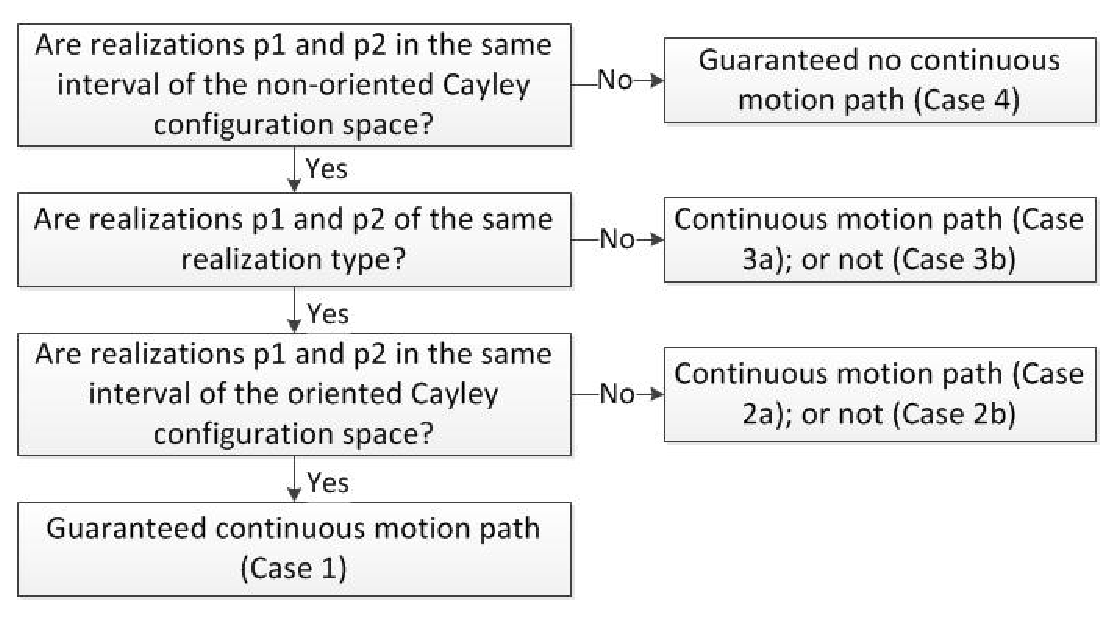
\includegraphics[width=.75\linewidth]{img/diagram}
\end{center}
\caption{Complete case analysis of continuous motion paths between two realizations $p_1$ and $p_2$. 
%Defining cases finding a continuous motion path between two realizations.
}
\label{fig:diagram}
\end{figure*}



%(2) Given a specific realization type, there is a linear time algorithm to convert 
%from a Cayley configuration $l_f$ to a corresponding realization.
%As we will see in Section \ref{sec:examples}, 
%lots of existing mechanisms can be converted to 1-dof tree-decomposable linkages with low Cayley complexity.
In \citeN{Sitharam2011a}, %we answer the following questions:  
algorithms are given for obtaining an (oriented) Cayley configuration space 
for generic 1-dof tree-decomposable linkages. 
Here a \emph{generic linkage} means that no bar length is zero, all bars have distinct lengths and 
at most one pair of adjacent bars can be collinear in any realization. 
A realization of a generic linkage automatically satisfies the usual notion of genericity in the rigidity literature.
It is also shown that for generic 1-dof tree-decomposable linkages with low Cayley complexity, 
the number of continuous motion paths between two realizations is \emph{at most two}, 
and can be directly obtained from the oriented Cayley configuration spaces with complexity linear
in a natural, discrete measure of the length of the path \cite[Theorem 3]{Sitharam2011a}.
%gave a set of local orientations, such that the Cayley configuration space only has a single interval and can be computed in $O(|V|^2)$ time if and only if this set of local orientations is specified, 

\citeN{Sitharam2011b} gives the following theorem for recognizing low Cayley complexity linkages:
\begin{theorem}[Four-cycle Theorem,  {\cite[Theorem 2]{Sitharam2011b}}]\label{the:four-cycle}
 A 1-dof tree-decomposable linkage has low Cayley complexity
if and only if every construction step of the underlying graph 
is based an adjacent pair of clusters, 
from a \emph{four-cycle} of clusters in the previously constructed graph. 
This yields an algorithm to recognize 1-dof tree-decomposable linkages with low Cayley complexity,
with time complexity quadratic in the number of construction steps of the underlying graph.
\end{theorem}
%
For example, the linkage in Figure \ref{fig:four_cycle}(b) does not have low Cayley complexity, 
since the construction step $v_3 \triangleleft (a,b)$ violates the four-cycle theorem: 
although  $v_3 \triangleleft (a,b)$ is based on the four-cycle of the four clusters $\triangle v_0v_1a$, $(v_1,v_0')$, $\triangle v_0'v_2b$, $(v_0,v_2)$, 
the  base clusters $\triangle v_0v_1a$ and $\triangle v_0'v_2b$ containing $a$ and $b$ are not adjacent in the four-cycle. On the other hand, the linkage in Figure \ref{fig:four_cycle}(b) satisfies the four-cycle theorem and  has low Cayley complexity.


%a recognition algorithm is given for 1-dof tree-decomposable linkages with low Cayley complexity,
%with time complexity quadratic in the number of construction steps of the underlying graph.


While judiciously chosen Cayley parameters  
shed light on many aspects of 1-dof tree-decomposable linkages,  
one persistent problem has been that %multiple Cartesian realizations correspond to the same Cayley configuration.
a non-oriented Cayley interval, being a union of multiple oriented Cayley intervals, 
could correspond to multiple connected components of the realization space. 
%as in Figure \ref{fig:beest_components}. 
%A single non-oriented Cayley interval is a union of multiple oriented Cayley intervals.
%The same example also shows that, 
On the other hand, although an oriented Cayley interval corresponds to a unique connected component, 
the mapping is not bijective, since that same connected component could contain more than one oriented interval \cite[Section 1.2]{sitharam2014beast}.
Figure \ref{fig:diagram} summarizes the different cases when 
determining existence of a continuous motion path between two realizations. 
There are two cases (2 and 3) where there may or may not exist a continuous motion path (a and b).
Previous software  
mentioned in Section \ref{sec:soa}, except for CUIK, 
generate continuous motion within a specified Cayley interval, 
or multiple segments of continuous motion, 
each corresponding to a different oriented Cayley interval with the same realization type. 
%, only looking at the Cayley intervals and realization types, 
Thus they cannot consistently distinguish Case 2a from Case 2b, %as shown in Figure xxx
or Case 3a from Case 3b. %as shown in Figure xxx.
The CUIK software deals with general mechanisms and 
provides comprehensive functionalities in continuous motion and connected components generation. %, distinguishing between these four types.
%uses a derivative tracing based algorithm to 
However, the derivative tracing numerical methods used by CUIK %deals with general linkages, 
must necessarily have non-polynomial complexity (unless P $=$ NP), 
%it could have high time complexity 
as opposed to the linear complexity algorithm \cite[Theorem 3]{Sitharam2011a} for linkages of low Cayley complexity.


\citeN{sitharam2014beast,Sitharam2011a} give a bijective representation to represent the realization space, 
by characterizing a \emph{canonical} method of picking a minimal set of non-edges, called a \emph{complete Cayley vector}, such that adding those non-edges as bars results in global rigidity.
The distance vectors on these non-edges (called \emph{complete Cayley distance vectors}) for each realization of the realization space form a \emph{canonical Cayley curve}, which bijectively represents the realization space.
In addition, the \emph{Cayley distance} between two Cartesian realizations is defined to be the Euclidean distance between their complete Cayley distance vectors,
and the \emph{Cayley distance} between two connected components is defined to be the minimum Cayley distance taken over all pair of realizations, one from each component. 
%which in turn provides a measure of distance between two connected components.
%a simple characterization is given for 1-dof tree-decomposable graphs with low Cayley complexity,
%yielding an efficient recognition algorithm. 

%show that (graph) planarity is equivalent to low Cayley complexity for a natural subclass of 1-dof tree-decomposable graphs. 




%Previous implementations only generate continuous motion for a fixed connected component, 
%or generate all realizations for a fixed realization type and a single user specified interval of the Cayley configuration space. 
%Thus, %we can see from Table \ref{table:cases} that 
%they 


%Based on these existing theoretical  contributions of \cite{Sitharam2011a,Sitharam2011b,sitharam2014beast}, 
In this paper, 
we present \texttt{CayMos}, a new system implementing these existing theoretical results
for configuration spaces analysis of 1-dof tree-decomposable linkages with low Cayley complexity.
%
Practical uses of \texttt{CayMos} include the following. 
(1) A substantial class of under-constrained systems occurring in mechanical CAD %TODO example 
 can be completed appropriately into
well-constrained systems, by providing the user with a comprehensive set of values (the Cayley configuration space) for additional constraints, that guarantee the existence of a solution for the augmented system. 
%
(2) A large class of 3D kinematic mechanisms are ``parallel'' 2D mechanisms based on common linkages 
such as the Strandbeest~\cite{jansen2009strandbeest}.
These mechanisms are used in robotics, self-deploying structures etc.
\texttt{CayMos} provides efficient and comprehensive analysis of their motions: connected components and continuous motion paths. 

In Section \ref{sec:contributions}, 
we list in detail the contributions of this paper in the form of \texttt{CayMos} functionalities. 
%\ref{sec:architecture}, 
We briefly describe the algorithms implemented in \texttt{CayMos} in Section~\ref{sec:algorithms}.
%\ref{sec:algorithms}, 
%and give the corresponding pseudocode in Section \ref{sec:pseudocode}. 
%In Section \ref{sec:classes} we describe the software architecture. 



\section{Contributions: CayMos functionality}
\label{sec:contributions}


Based on the theoretical  contributions of \citeN{Sitharam2011a,Sitharam2011b,sitharam2014beast}, 
we present software package, \texttt{CayMos} \citep{bib:caymos} (source code and user manual available at http://calgo.acm.org/), 
which implements efficient algorithmic solutions for the following: 
%provides efficient implementation of the algorithms from \cite{Sitharam2011a,Sitharam2011b,sitharam2014beast} 

\noindent\textbf{(1)} Determining low Cayley complexity and generating Cayley configuration spaces for a given linkage,
implementing \cite[Section B]{Sitharam2011a} and \cite[Theorem 2]{Sitharam2011b}.

\noindent\textbf{(2)} Meaningfully visualizing the %Cayley distance vector, and visualizing 
connected components of the realization space as projection of the canonical Cayley curves, 
implementing \cite[Theorem 3]{sitharam2014beast}, addressing Issue (a) from Section \ref{sec:soa}.
%on three non-edges picked by the user from the complete Cayley vector. 

\noindent\textbf{(3)} Generating the connected components of the realization space, 
and finding a continuous motion path between two given realizations, 
implementing \cite[Theorem 3]{Sitharam2011a} and \cite[Theorem 5(i)]{sitharam2014beast}, addressing Issue (b) from Section \ref{sec:soa}.
%(i) the connected component containing current realization, 
%(ii) all connected components of the realization space. 

\noindent\textbf{(4)} Finding the realizations representing the shortest Cayley distance between two different connected components of the realization space, 
implementing \cite[Theorem 5(ii)]{sitharam2014beast}, addressing Issue (c) from Section \ref{sec:soa}.
%For two given realizations  
%(i) in the same connected component: find a continuous path between them, 
%with or without fixing a realization type; 
%(ii) in different connected components: 
%find the two nearest realizations from the two components.

In the following we will briefly introduce the functionalities provided by \texttt{CayMos}.

\smallskip

Screen-shots and movies generated by \texttt{CayMos}  may be found in  \citeN{sitharam2014beast,Sitharam2011a}.
%to illustrate definitions and theoretical results. 
%However this manuscript provides the first description of \texttt{CayMos} functionalities and architecture. 






%-----------------------

\subsection{Determining low Cayley complexity and generating Cayley configuration spaces}\label{subsec:ccs}
% 
%\begin{figure*}[tp]
%\begin{center}
%\includegraphics[width=1.1\linewidth]{img/ccs}
%\end{center}
%\caption{Generating the non-oriented Cayley configuration space of the Limacon linkage using \texttt{CayMos}. 
%(A) Button for generating the Cayley configuration space. 
%(B) Spinner for specifying the length of the base non-edge and showing the corresponding realizations. % navigating the Cayley configuration space. 
%(C) Intervals of the Cayley configuration space. The black dot denotes the Cayley configuration for the current realization. }
%\label{fig:ccs}
%\end{figure*}
%
%\texttt{CayMos} accepts user input of a linkage by 
%allowing the user to draw the bar and joints of the linkage. 
As  Contribution (1), 
the user can generate the Cayley configuration spaces for 1-dof tree-decomposable linkages with low Cayley complexity. 
The following functionalities are provided: %by \texttt{CayMos}, implementing Contribution Item (1): 

\noindent(\romannumeral 1) Determining whether the given linkage is 1-dof tree-decomposable with low Cayley complexity. % implementing the Four-cycle algorithm \cite{Sitharam2011b}. 

\noindent(\romannumeral 2) Generating both the oriented and non-oriented Cayley configuration space(s)
for a linkage with low Cayley complexity. 
%implementing the ELR algorithm \cite{Sitharam2011a}.
The user can change the length of the chosen base non-edge to see corresponding realizations, as well as specify the realization type.

See Figure~1 in the user manual~\cite{userman} for an annotated illustration of the user interface.
 

\subsection{Visualizing the connected components and finding continuous motion paths of the realization space}\label{subsec:connected_component}
%
%\begin{figure*}[tp] 
%%\vspace{-80pt}
%%\begin{subfigure}[b]{\linewidth}
%\begin{center}
%\includegraphics[width=1.05\textwidth]{img/component1}
%\end{center}
%\caption{Finding the connected components and showing corresponding canonical Cayley curves of 
%the Limacon linkage using \texttt{CayMos}. %, where (Fig.a) and (Fig.b) show two different connected components. 
%(A) Button for generating the connected components. 
%(B) The current realization, moving as the user traces the connected component. Dashed non-edges: non-edges in the complete Cayley vector. 
%(C) Panel showing the complete Cayley distance vector for current realization. 
%%\texttt{CayMos} allows the user to pick three non-edges for 3D projection of the canonical Cayley curve,  
%%where the picked non-edges are shown in red, green and blue in (B) and (C). 
%(D) Spinner for tracing the current connected component. 
%(E) Button for showing the 3D projection of the corresponding canonical Cayley curve. 
%(F) Spinner for navigating all connected components in the realization space. 
%(G) The 3D projection of the canonical Cayley curve of the current component. 
%The dot denotes the current realization and moves as the user traces the connected component. 
%The curve is color-coded according to realization types. 
%(H) The intervals of the oriented Cayley configuration spaces contained in the current connected component. }
%\label{fig:components}
%\end{figure*}
%

%After generating the Cayley configuration space, 
As Contribution (2) and (3),
the user can generate and visualize the connected components of the realization space,  
as well as find a continuous motion path between two realizations. 
The following functionalities are provided: % by \texttt{CayMos}, implementing Contribution Item (2) and (3): 

\noindent(\romannumeral 1) Showing the non-edges in the complete Cayley vector of the linkage, 
as well as displaying the complete Cayley distance vector for the current realization. 
%See Figure \ref{fig:components} (B) and (C). 

\noindent(\romannumeral 2) Generating all the connected components of the realization space,
as well as finding a continuous motion path (if one exists) between two realizations specified by the user.
%See Figure \ref{fig:components} (A) and (F). 

\noindent(\romannumeral 3) Visualizing the connected component by showing the corresponding canonical Cayley curve, projected on three non-edges picked by the user from the complete Cayley vector. 
%\texttt{CayMos} permits the user to use a spinner to trace the connected component, 
%and a moving dot is shown on the curve to denote the current realization.
%The canonical Cayley curve is color-coded corresponding to realization types encountered in the connected component. 
%See Figure \ref{fig:components} (E), (G) and (D). 
%Visualizes the connected component by  showing the projection of the


%\noindent(\romannumeral 4) Showing the intervals of oriented Cayley configuration spaces contained in the current connected component. 
%The intervals are color-coded corresponding to realization types. 
%See Figure \ref{fig:components} (H). 

\noindent(\romannumeral 4) Showing the curves traced out by vertices of the linkage in continuous motion. 


See Figure~3 in the user manual~\cite{userman} for an annotated
screen-shot highlighting the functionalities described
in (i), (ii) and (iii) above.



\subsection{Cayley distance between connected components}\label{subsec:distance}


As Contribution  (4), 
when the user tries to find a continuous motion path between two realizations in different connected components, 
\texttt{CayMos} will
%generate the connected components for both realizations and 
find the two nearest realizations of these two components.
%implementing  Contribution Item (4). 
%Both connected components are shown as projected curves, 
%and the two nearest realizations are marked on the two curves. 
%See Figure \ref{fig:nopath}. 


%\section{\texttt{CayMos} software architecture and pseudocode}
%\label{sec:architecture}

\section{Algorithms implemented in CayMos}
\label{sec:algorithms}

%(existed; clear, brief simple description. can briefly mention QIM. General technique. quick complexity analysis. )
Several algorithms from our previous papers \citeN{Sitharam2011a,Sitharam2011b,sitharam2014beast} are implemented in \texttt{CayMos}. 
Here we give a brief description of these algorithms. 



\textbf{Four-cycle algorithm}: to determine whether a given 1-dof tree-decomposable linkage has low Cayley complexity, 
we implement the \emph{Four-cycle algorithm} \cite[Theorem 2]{Sitharam2011b},
which follows the construction of the linkage, and tests whether each construction step 
satisfies the condition given by the Four-cycle Theorem (see  Section \ref{sec:previous_cayley}).
%is based on 
%an adjacent pair from a \emph{four-cycle} of clusters in the previously constructed graph. 
For each of the $O(|V|)$ construction steps, we need to check $O(|V|)$ candidate base pairs of clusters, so
the overall time complexity is $O(|V|^2)$, 
%\noindent (1) Add all adjacent cluster pairs in the first level to $L$. 
%\noindent (2) For each subsequent construction step $v_{k}\triangleleft(u_{k}\in T_k,w_{k}\in T_k')$, do:
%\begin{enumerate}
%\item Find the following two sets of clusters: $U=\{T_{u}|T_{u}\in G_{f}(k-1),u_{k}\in T_{u}\}$,
%$W=\{T_{w}|T_{w}\in G_{f}(k-1),w_{k}\in T_{w}\}$.
%\item Find all the pairs $(T_{u},T_{w})\in U\times W$ such that %$T_{u}\cap T_{w}\neq\emptyset$ and 
%$(T_{u},T_{w})$ is in $L$; if no such pair exists, return that $G$ does not have low Cayley complexity. 
%\item For all the pairs $(T_{u},T_{w})\in U\times W$ such that $T_{u}\cap T_{w}\neq\emptyset$,
%add $(T_k,T_{u})$ and $(T_k',T_{w})$ to $L$. Add $(T_k,T_k')$ to $L$.
%\end{enumerate}
%Let $n$ be the total number of construction steps. 
%Step (1) takes $O(n^2)$ time. 
%For each iteration of Step (2), Substep 1 takes $O(d_u+d_k)$ time, Substep 2 takes $O(d_ud_k)$
%time, step 3 takes $O(d_ud_k)$ time, where $d_u = cdeg(u_k)$, $d_w = cdeg(w_k)$. % is the $cdeg$ of $u_k$ and $w_k$. 
%Therefore the overall time complexity is $O(n^2)$. 

\textbf{ELR algorithm}: 
to find the Cayley configuration space of a 1-dof tree-decomposable linkage with low Cayley complexity, 
we implement the \emph{ELR (extreme linkage realization) algorithm} \cite[Section B]{Sitharam2011a}.
The algorithm works by realizing all the \emph{extreme linkages} consistent with each realization type, 
and finding the intersection of all the candidate intervals of the base non-edge. 
%Realizing each extreme linkage takes time $O(n)$. 
The overall time complexity is exponential in $|V|$.
As the problem of computing the Cayley configuration space is NP-hard \citep[Observation 2]{Sitharam2011a},
an improvement over exponential time complexity is unexpected unless P $=$ NP. 
\citeN{Sitharam2011a} also contains another algorithm called \emph{QIM (quadrilateral interval mapping)}, which also computes the Cayley configuration space, 
but only applies to a special subclass of linkages called \emph{1-path} 1-dof tree-decomposable linkages. 
The implementation of QIM algorithm is not included in \texttt{CayMos}. 


\textbf{Continuous motion algorithm}: 
to find continuous motion paths and connected component(s) of the realization space, we implement the \emph{Continuous motion  algorithm} \cite[Theorem 3]{Sitharam2011a}, \cite[Theorem 5(i)]{sitharam2014beast}.
The algorithm works by traversing the intervals in the oriented Cayley configuration space via the common interval endpoints. 
As mentioned in Section \ref{sec:previous_cayley},
the time complexity is linear in the number of oriented Cayley configuration space endpoints along the continuous motion path or connected component. 

%For (i), the following algorithm finds a path of continuous motion between two realizations in time linear in the number of endpoints along that path: 
%From the starting realization $G(p_s)$ with forward realization type $\sigma$, 
%we take the oriented Cayley configuration space for realization type $\sigma$ and find the interval $I_\sigma$ that $G(p_s)$ is in. 
%By Lemma \ref{lem:endpoint} (i), inside $I_\sigma$ there always exists a path of continuous motion. 
%Take one endpoint $l_f = l_0$ of $I_\sigma$. 
%In the corresponding realization $G(p_0)$, exactly one entry, say entry $i$, of the forward realization type is $0$. 
%By Lemma \ref{lem:reachable}, 
%the next immediately reachable oriented Cayley configuration space is uniquely determined, 
%since its realization type $\tau$ should be the same as $\sigma$ except having the opposite sign in entry $i$.
%Since intervals in an oriented Cayley configuration space are all disjoint, 
%there is at most one interval in the oriented Cayley configuration space for realization type $\tau$ 
%with $l_0$ as an endpoint. So 
% we can find at most one interval $I_\tau$ immediately reachable. 
%We repeat the process from the other endpoint of $I_\tau$ until we reach the interval containing the target realization, or we may arrive at a deadend, in that case we start again from the other endpoint of $I_\sigma$.  
%Each endpoint encountered leads to at most one next immediately reachable interval, so backtracking is never necessary.
%Therefore the time complexity is linear in the number of endpoints along the path we found.
%Since both endpoints of $I_\sigma$ could potentially lead to the target realization, 
%there are \emph{at most two paths} between two given realizations. 


\textbf{Closest pair algorithm}: 
to find the pair of ``closest'' realizations between two different connected components, 
we implement the \emph{Closest pair algorithm} \cite[Theorem 5(ii)]{sitharam2014beast},
%We use the Continuous motion algorithm to find the oriented Cayley configuration space intervals of both two connected component, 
which samples both components and returns the pair of realizations with the smallest Cayley distance, %from each component. 
which is computed using the complete Cayley distance vector (see Section \ref{sec:previous_cayley}).


\medskip


The backend of CayMos consistes of two parts:
     a) 1-dof tree decomposable linkages and Cayley
        configuration spaces, and
     b) continuous motion generation and representation.
    The major classes and methods within each of these areas
    are described in further detail in the user manual that
    accompanies the software component~\cite{userman}.


\medskip
\noindent \textbf{Note}: The source code and user manual of \texttt{CayMos} are available at http://calgo.acm.org/.


%\subsection{Major classes and architecture of \texttt{CayMos}}
%\label{sec:classes}
%
%
%
%Overall the backend of \texttt{CayMos} consists of two parts, with the following major classes. 
%%The backend of the system can be divided into two parts: 
%
%
%\subsubsection{1-dof tree-decomposable linkages and Cayley configuration spaces}
%
%
%\begin{enumerate}
%
%
%\item The \textsf{TDLinkage} class: represents a 1-dof tree-decomposable linkage. 
%%Determines whether a linkage has low Cayley complexity, and generates the Cayley configuration space.
%
%
%
% Major Attributes:
%
%\noindent --  \textsf{graph}: the underlying graph of the linkage. 
%
%\noindent --  \textsf{barLengths}: the length of the bars of the linkage. 
%
%\noindent --  \textsf{baseNonedge}: current base non-edge of the linkage.
%
%\noindent --  \textsf{completeCayleyVector}: the complete Cayley vector for the current base non-edge.
%
%\noindent --  \textsf{cayleyConfigurationSpace}: the Cayley configuration space on the current base non-edge. 
%
%\smallskip
%\noindent Major Methods:
%
%\noindent-- \textsf{isLow()}: elaborated in Section \ref{sec:islow}.
%
%\noindent-- \textsf{getCayleyConfigurationSpace()}: elaborated in Section \ref{sec:getcayleyconfigurationspace}.
%
%
%\item The \textsf{Realization} class: represents a realization of a \textsf{TDLinkage} instance.
%
%\noindent Major Attributes:
%
%\noindent --  \textsf{tdLinkage}:
%the corresponding 1-dof tree-decomposable linkage of the realization. 
%
%\noindent --  \textsf{points}:
%the 2D points in the realization for the vertices of the linkage. 
%
%\smallskip
%
%\noindent Major Methods:
%
%\noindent --  \textsf{length(e:Edge)}: 
%Returns the length of \textsf{e} in the realization, where \textsf{e} can be an edge or a non-edge.
%
%\noindent --  \textsf{getCompleteCayleyDistanceVector}(): 
%Returns the complete Cayley distance vector of the realization.
%Calls \textsf{length()} for each non-edge in the \textsf{completeCayleyVector} field of \textsf{tdLinkage}, with time complexity $O(|V|)$.
%
%\noindent --  \textsf{cayleyDistance(that:Realization)}: 
%Returns the Cayley distance \cite[Section 3.2]{sitharam2014beast} between this realization and \textsf{that} with time complexity $O(|V|)$.
%
%
%
%\item The \textsf{CayleyConfigurationSpace} and \textsf{OrientedCayleyConfigurationSpace} classes: represent the Cayley configuration space of a \textsf{TDLinkage} instance. Each \textsf{CayleyConfigurationSpace} contains multiple \textsf{OrientedCayleyConfigurationSpace} instances. 
%
%\item The \textsf{OrientedInterval} class: represents an interval in an oriented Cayley configuration space. 
%
%\noindent Major Attributes:
%
%\noindent -- \textsf{upper} and \textsf{lower}:
%the upper and lower endpoints of the interval.
%
%\noindent --  \textsf{realizationType}:
%the realization type of the \textsf{OrientedCayleyConfigurationSpace} containing the interval.
%
%\noindent --  \textsf{nextIntervalUpper} and \textsf{nextIntervalLower}:
%the two \textsf{OrientedInterval} instances sharing a common endpoint with this interval. 
%They are immediately reachable from this interval in a continuous motion.
%
%
%\end{enumerate}
%
%
%
%%\item CayleyConfigurationSpace: the Cayley configuration space of a TDLinkage instance on a base non-edge. 
%\subsubsection{Continuous motion generation and representation}
%
%\begin{enumerate}
%
%
%\item The \textsf{ContinuousMotion} class: represents a continuous motion path between two \textsf{Realization} instances, or a connected component of a \textsf{TDLinkage} instance. 
%
%
%\noindent  Major Attributes:
%
%\noindent -- \textsf{tdLinkage}: 
%the corresponding 1-dof tree-decomposable linkage of the continuous motion. 
%
%\noindent --  \textsf{orientedIntervals}: 
%the list of \textsf{OrientedInterval} instances encountered along the continuous motion.
%
%\smallskip
%
%\noindent Major methods:
%
%\noindent -- \textsf{findComponent()}, \textsf{findPath()} and \textsf{findAllComponents()}: elaborated in Section~\ref{sec:findpath}.
%
%\noindent -- \textsf{findNearestRealizations()}: elaborated in Section~\ref{sec:findnearest}.
%
%
%\noindent -- \textsf{getRealizations()}: 
%Returns a list of realization samples along the continuous motion by sampling the \textsf{orientedIntervals} field. 
%Uses a sampler object so that different ways of sampling can be chosen at runtime. 
%
%\noindent --  \textsf{get3DCurve(f1,f2,f3)}: 
%Returns a \textsf{Curve3D} instance representing the 3D projection of the continuous motion's corresponding Cayley curve
%on \textsf{f1}, \textsf{f2} and \textsf{f3}, three non-edges from the complete Cayley vector of tdLinkage. 
%The time complexity is linear in the size of the list returned by \textsf{getRealizations()}.
%
%
%\item The \textsf{Curve3D} class: supports visualization of a  \textsf{ContinuousMotion} instance as a Cayley curve projected in 3D.
%
%\end{enumerate}
%
%\begin{figure*}[tp]
%\begin{center}
%\includegraphics[width=1.1\linewidth]{img/uml}
%\end{center}
%\caption{UML diagram for major classes. }
%\label{fig:uml}
%\end{figure*}
%
%Figure \ref{fig:uml} shows the relationships between the above classes. 
%
%
%
%
%

%\subsection{Major methods implementing algorithms in Section~\ref{sec:algorithms}}
%\label{sec:pseudocode}
%
%\subsubsection{ Method \textsf{isLow()}} %implements the Four-cycle algorithm \cite{Sitharam2011b} sketched in Section \ref{sec:algorithms}
%\label{sec:islow}
%
%%Returns whether the linkage \textsf{this} has low Cayley complexity. 
%%Initializes the \textsf{completeCayleyVector} field, % for linkages with low Cayley complexity,
%%which stores the complete Cayley vector for the current base non-edge. 
%
%The method implements the Four-cycle algorithm \cite[Theorem 2]{Sitharam2011b} sketched in Section \ref{sec:algorithms} to determine low Cayley complexity,
%returning \textsf{true} if the calling \textsf{TDLinkage} instance has low Cayley complexity, or \textsf{false} otherwise.
%It also implements  \cite[Theorem 3]{sitharam2014beast} to find the complete Cayley vector
%and store it in  the  \textsf{completeCayleyVector} field. 
%Since both algorithms follow the construction of the linkage, we combine the implementation into one method. 
%The  time complexity is $O(|V|^2)$. 
%
%\smallskip
%\noindent\textbf{Note:} in the current version of the software, the complete Cayley vector is implemented 
%as in \cite[Theorem 3]{sitharam2014beast}, which is not minimal. 
%The \emph{minimal complete Cayley vector} introduced in \cite[Theorem 4]{Sitharam2011a} will have dimension two for a large number of 1-dof tree-decomposable linkages. 
%
%\smallskip
%
%\lstset{language=Java} 
%
%\lstset{
%  language=Java,
%  tabsize=2,
%  basicstyle=\footnotesize\sffamily,
%  %frame=single,
%  breaklines=true
%}
%
% Pseudocode for  \textsf{isLow()} :
%
%\begin{lstlisting}[mathescape]
%boolean isLow() {
%	completeCayleyVector.add(baseNonedge);
%
%	for (each construction step s) {
%	// Construction Step s: adding two clusters s.c1 and s.c2, s.v $\triangleleft$ (s.v1, s.v2), s.v1 $\in$ s.c1, s.v2 $\in$ s.c2
%		if (s is not directly based on the base non-edge) { 
%			// find a valid pair of base clusters
%			for (each Vertex w in the previously constructed graph sharing a cluster with both $s.v1$ and $s.v2$){
%				Cluster c1 = the cluster containing s.v1 and w;
%				Cluster c2 = the cluster containing s.v2 and w;
%				if (validBasePairs.contains((c1,c2)){
%					isLowStep = true;
%					completeCayleyVector.add(nonedge (w, s.v));
%					currentBasePairs.add((c1,c2));
%				}
%			}
%
%			if (!isLowStep)  // does not have low Cayley complexity
%				return false;
%
%			for (Pair(c1,c2) in currentBasePairs){
%				validBasePairs.add((s.c1, c1));
%				validBasePairs.add((s.c2, c2));
%			}
%		}
%		validBasePairs.add((s.c1,s.c2));
%	}
%	return true;
%}
%\end{lstlisting}
%
%
%
%\subsubsection{ Method \textsf{getCayleyConfigurationSpace()}}
%\label{sec:getcayleyconfigurationspace}
%The method implements the ELR algorithm \citep{Sitharam2011a} sketched in Section \ref{sec:algorithms}
%%
%to generate and return the %\textsf{CayleyConfigurationSpace} instance
%Cayley configuration space of the calling \textsf{TDLinkage} instance on the current base non-edge. 
%%nitializes the field \textsf{cayleyConfigurationSpace}. 
%%Implements the ELR algorithm \cite{Sitharam2011a}. 
%The generated Cayley configuration space is also stored in the \textsf{cayleyConfigurationSpace} field
%of the calling \textsf{TDLinkage} instance.
%As pointed out in \citeN{Sitharam2011a}, computation of the Cayley configuration space is NP-hard, and this method can take time exponential in $|V|$.
%
%\smallskip
% Pseudocode for  \textsf{getCayleyConfigurationSpace()} :
%
%\begin{lstlisting}[mathescape]
%CayleyConfigurationSpace getCayleyConfigurationSpace() {
%	for (each construction step s) {
%		for (each extreme linkage Realization r at step s) {
%			distance = r.length(baseNonedge);
%			for (each complete solution type t compatible with the partial solution type of r) 
%				candidateEndpointLists[t].add(distance);
%		}
%	}
%	
%	for ( (SolutionType:t,List:l) : candidateEndpointLists) {
%		sort(l);
%		occs = new OrientedCaylyConfigurationSpace with SolutionType t;
%		for (double cur : l) {
%			double prev = the point before cur in l;
%			double next = the point after cur in l;
%			boolean P = realizable((prev + cur) / 2, t);
%			boolean N = realizable((cur + next) / 2, t);
%			if (!P && !N) {
%				// cur is an isolated point
%				occs.appendInterval(cur, cur); 
%			} else if (P && !N) {
%				// cur is end of interval
%				occs.appendInterval(lastEndpoint, cur); 
%				intervalStart = null;
%			} else if (!P && N){
%				// cur is start of interval
%				intervalStart = cur; 
%			} // else: cur is in middle of interval
%		}
%		this.cayleyConfigurationSpace.addOrientedCayleyConfigurationSpace(occs);
%	}
%	return this.cayleyConfigurationSpace;
%}
%\end{lstlisting}
%
%
%\subsubsection{Methods \textsf{findPath(r1:Realiztion, r2:Realization)}, \textsf{findComponent(r:Realization)}, \textsf{findAllComponents(l:TDLinkage)} } \label{sec:findpath}
%These methods implement the Continuous motion algorithm \cite[Theorem 3]{Sitharam2011a} sketched in Section \ref{sec:algorithms}.
%%
%%
%Method \textsf{findPath(r1,r2)} 
%returns an instance of \textsf{ContinuousMotion}
%representing the continuous motion path between realizations \textsf{r1} and \textsf{r2}, 
%which are realizations of the same linkage. 
%Method \textsf{findComponent(r)} returns an instance of \textsf{ContinuousMotion}, 
%which is the connected component in the realization space containing the realization \textsf{r}. 
%%in the realization space of \textsf{r}'s corresponding linkage.
%%It also initializes the \textsf{orientedIntervals} field of \textsf{r}.
%Method \textsf{findAllComponents(l)}
%returns a list of \textsf{ContinuousMotion} instances representing all connected components in the realization space of the linkage \textsf{l}. 
%
%Both \textsf{findPath()} and \textsf{findComponent()}  %implement the Continuous motion algorithm \cite{Sitharam2011a}, 
%have time complexity linear in the number of oriented Cayley configuration space endpoints contained in the 
%\textsf{ContinuousMotion} instance returned. 
%Method \textsf{findAllComponents()} %also implements Theorem 5 from \cite{sitharam2014beast}, 
%has time complexity linear in the total number of endpoints of all oriented Cayley configuration spaces \cite[Theorem 3]{sitharam2014beast}. 
%
%\smallskip
% Pseudocode for \textsf{findComponent()} (\textsf{findPath()} is implemented similarly):
%\begin{lstlisting}
%static ContinuousMotion findComponent(Realization r) {
%	startInt = the OrientedInterval containing the Cayley configuration of r;
%	component.orientedIntervals.add(startInt);
%
%	OrientedInterval curInt = startInt; 
%	double endlf = curInt.lower;
%	while (true) {
%		curInt = (endlf == curInt.lower? curInt.nextIntervalLower:curInt.nextIntervalUpper)
%		if (curInt == startInt) 
%			return component;	
%		endlf = (endlf == curInt.lower? curInt.upper:curInt.lower);
%		component.orientedIntervals.add(curInt);
%	}
%}
%\end{lstlisting}
%
%The method  \textsf{findAllComponents()} is implemented by iterating over all intervals 
%in every \textsf{OrientedCayeyConfigurationSpace} and 
%calling \textsf{findComponent}.
%
%
%%\noindent High level sourcecode for  \textsf{findAllComponents()}:
%%
%%\begin{lstlisting}
%%List findAllComponents(TDLinkage t) {
%%	for (OrientedCayleyConfigurationSpace oc : t.getCayleyConfigurationSpace()) 
%%		intervalSet.add(oc.orientedIntervals);
%%
%%	while (!intervalSet.isEmpty()) {
%%		OrientedInterval inv = an oriented interval from intervalSet;
%%		ContinuousMotion component = find the component containing inv;
%%		componentsList.add(component);
%%
%%		for (OrientedInterval n : component.orientedIntervals) 
%%			intervalSet.remove(n);
%%	}
%%	return componentsList;
%%}
%%\end{lstlisting}
%
%
%\subsubsection{Method \textsf{findNearestRealizations(c1: ContinuousMotion, 
% c2: ContinuousMotion)}}\label{sec:findnearest}
% The method implements the Closest pair algorithm \cite[Theorem 5(ii)]{sitharam2014beast}
% sketched in Section \ref{sec:algorithms}.
% %
%The method returns the pair of two nearest realizations between the two connected components 
%\textsf{c1} and \textsf{c2} of the realization space of a linkage, 
%using the Cayley distance measure. 
%%
%%Implements Theorem 5 from \cite{sitharam2014beast}, 
%The time complexity $O(k^2|V|)$, 
%where $k$ is the size of the list returned by \textsf{getRealizations()},
%which is a  list of sample realizations in the connected component.
%%Uses the completeCayleyDistanceVectors field of both c1 and c2. 
%
%%\smallskip
%%Pseudocode for \textsf{findNearestRealizations()}:
%%
%%\begin{lstlisting}
%%static Pair findNearestRealizations(ContinuousMotion c1, ContinuousMotion c2) {
%%	double nearestDistance = Double.POSITIVE_INFINITY;
%%	Realization result1 = null, result2 = null;
%%	for (Realization r1 : c1.getRealizations()) {
%%		for (Realization r2 : c2.getRealizations()) {
%%			double dis = r1.cayleyDistance(r2);
%%			if (dis < nearestDistance) {
%%				result1 = r1; result2 = r2;
%%				nearestDistance = dis;
%%			}
%%		}
%%	}
%%	return (result1, result2);
%%}
%%\end{lstlisting}
%
%
%
%%Their major attributes and methods are described 
%%in the following subsections. % we describe in detail the above classes with their attributes and methods. 
%
%
%
%%which is not the minimal complete Cayley vector as in \cite{Sitharam2011a}.
%
%
%







%\bibliographystyle{authordate1}
\bibliographystyle{ACM-Reference-Format-Journals}
\bibliography{readings}

\received{Month Year}{Month Year}{Month Year}

\end{document}
